\section{Definitions}\label{sec:methods}
The toy objective is
\begin{equation}
\mathcal{L}=\mathcal{L}_1+\lambda\mathcal{L}_2,\qquad\lambda=0.5.
\label{eq:objective}
\end{equation}
The encoder maps inputs to an embedding space; a separate generative model
samples a latent space. These terms are retained as distinct definitions.
No causal or universal performance claim is supplied.
\begin{figure}[htbp]
\centering
\begin{minipage}{0.8\linewidth}
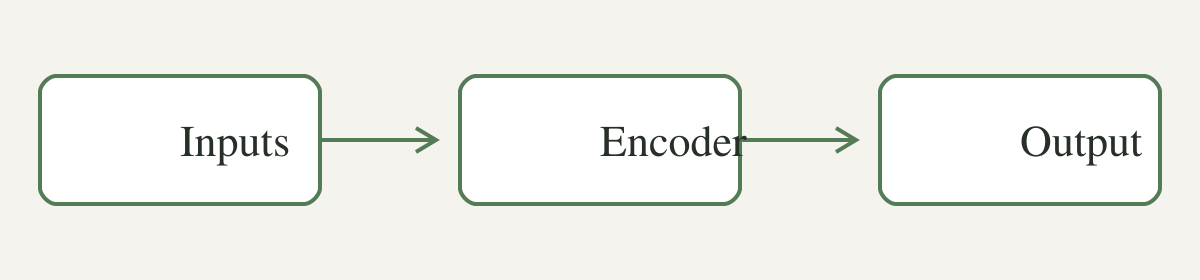
\includegraphics[width=\linewidth]{figures/panel}\\
\small (a) Supplied schematic
\end{minipage}\par\medskip
\begin{minipage}{0.8\linewidth}
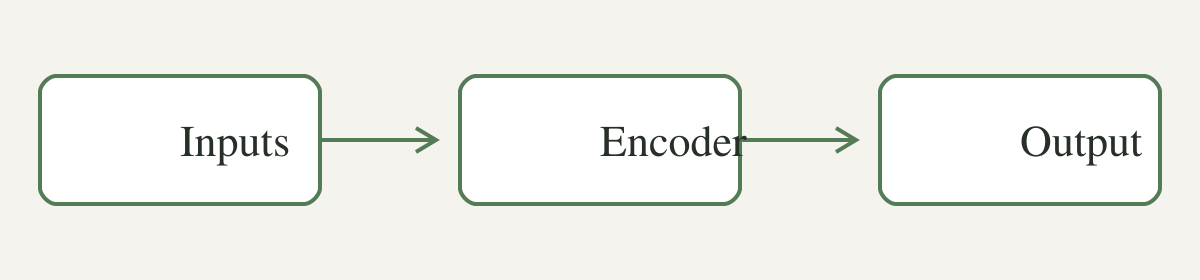
\includegraphics[width=\linewidth]{figures/panel}\\
\small (b) The same illustrative pipeline
\end{minipage}
\caption{Two synthetic panels; neither implies measured model behavior.}
\label{fig:panels}
\end{figure}
